\section{Introdução}

Atualmente possuímos redes sem fios em praticamente qualquer lugar, porém ainda há locais onde as transmissões usando ondas eletromagnéticas não são desejáveis. Como por exemplo em voos e hospitais, devido às possíveis interferências nos aparelhos do hospital ou na comunicação do avião com a torre. Outro local onde a radiofrequência não é muito utilizada é debaixo d'água, devido a alta condutividade elétrica da água, assim prejudicando a transmissão.

Uma forma para resolver os problemas citados acima seria uma nova forma de transmissão de dados e um forte candidato para isso é o VLC (Visible Ligth Communication). Que é um sistema de comunicação por luz visível, ou seja, modula a informação e a transmite informações na faixa do espectro que varia entre 390 nm a 700nm.

\begin{figure}[h]
  \centering
  \caption{Espectro eletromagnético}
  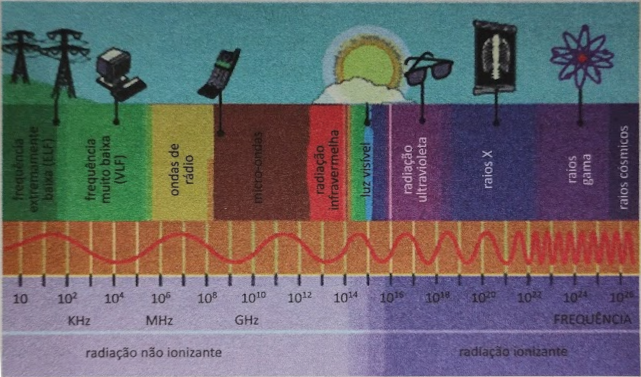
\includegraphics[width=0.8\textwidth]{images/espectro_eletromagnetico.png}
  
  \legend{Fonte: \citeonline[p. 9]{ondas}}
\end{figure}


Um dos pontos que fazem o VLC ser uma solução é o baixo custo, pois utiliza leds para a comunicação. Tal componente tem alta durabilidade e baixo consumo de energia, além de ser possível aproveitar a luz na iluminação no caso de um ambiente fechado, já que a transmissão é muito veloz a variação da iluminação é imperceptível ao olho humano.
